\section*{Background}
% 1M skyldes lønn til mennesker eller kun compute? (tid = penger hvis det er
% mennesker)

% BF: Har du en referanse vi kan bruke her? Dette er en ganske vanlig quote, men
% husker ikke hvor jeg har sett den, Dette er veldig generelle greier, men vi
% skulle hatt et par gode paper å sitere. 
In the past decade the generation of biological datasets has been unprecedented,
and the famous "\$1000k genome, \$1M analysis"\cite{} has become more apparent.
% mer om biologi og data 

% Trenger litt tekst som sier at vi skal snakke om stats, presentasjon, dbs,
% microservices og kobling av alle. 

% R og stats 
To analyze the growing biological data sets, there is now a number of analysis
tools in various programming languages.\cite{} In R, there are popular package
repositories such as CRAN \url{cran.r-project.org} or Bioconductor
\url{bioconductor.org} where developers can share software packages and keep
them up-to-date.  These repositories contain software packages for exploring
high-throughput genomic data in one environment. This includes both
pre-processing, e.g. cleaning, removing outliers, and analysing it with known
statistical methods. In other languages such as Python or Go developers can
choose bioinformatics libraries such as BioPython\cite{} and biogo\cite{}
respectively.  However all of these software packages require users to have a
high level of coding skills. 

% Vis 
A key part of analysing biological data is to visualize it. Researchers often
start data analysis by using simple visualization techniques to get a quick
overview of the data. Continuing in the data analysis pipeline researchers can
use more advanced visual techniques to explore the data either using
software packages or complete data visualization applications. Traditionally
data visualization applications have been built as desktop applications that
require installation and setup by the user, but now the move is towards software
that run in the web browser without any user setup. 

% Data fra R til vis
To visualize and share results from statistical analyses, the results are often
exported to a data format such as comma-separated values (CSV) and
then visualized using an external tool. This decouples data presentation and
analysis.  Through initiatives such as ApacheR and OpenCPU there has been a move
towards embedding scientific computation in data visualization application. This
removes the decoupling of statistical frameworks and interaction with the
analysis results. 

% Koble data sammen med db. 
Interpreting the analysis results require integration of known biology, either
from biological databases such as MSigDB\cite{} or KEGG\cite{}, or through
scientific publications from reference databases such as PubMed\cite{}.
Performing manual lookup into these databases is often tedious and error-prone,
making it necessary to automate the task. Now as more databases provide REST
APIs it is possible to provide software packages for automatic retrival of
database information. 

% Hvorfor bryr vi oss om både stats + DBs?  Skal vi si noe om at det blir
% vanligere å bruke REST APIs fremfor å laste ned alt og lese ting lokalt

% Her ser det ut som teksten er work-in-progress, siden de neste 4 § sier
% omtrent det samme

% Lage apps som gjør alt dette. 

% Hva er micro-services? 
Microservice architectures structures applications into small reusable, loosely
coupled parts. These communicate via lightweight programming language-agnostic
protocols such as HTTP, making it possible to write single applications in
different programming languages. This makes it possible to use the most suitable
programming language for each specific part. E.g. to use R and Bioconductor to
analyse biological data, or C++ and OpenCV for high-performance computer vision
tasks, or HTML, CSS, and JavaScript to build portable user-interfaces. 

% WIP WIP WIP
In systems biology there is a need for visualization tools that can make use of
the lastest statistical packages and interact with these. It is not enough to
visualize the results of an analysis pipeline, but interact with the different
steps from the final visualization. Examples of this interaction can be
modifying clustering parameters that are used in the analysis.

\subsubsection*{Requirements} 
From our experience building data exploration applications we have  ... the
following requirements 

\begin{enumerate}
    \item A language-independent approach for integrating, or embedding,
        statistical software, such as R, directly in interactive data
        exploration applications.
    % Ikke motivert behovet for up-to-date
    \item A 
        
        Up-to-date interfaces to online databases providing meta-data for
        understanding results from statistical analyses.
    % Ikke sagt noe om maintance & deployment
    \item Ease of software development, maintenance and deployment. 
\end{enumerate} 

\subsubsection*{Contributions} 
Our contributions are: 
\begin{enumerate}
% men ikke visualization?
\item An approach for developing data exploration applications for systems
biology that combine statistical analyses with online databases.  
\item A demonstration of its viability through N different applications. 
\item Performance evaluation of its central data analysis component. 
\end{enumerate} 


\subsection*{Related Work} 
% Hva er korrekt: "in" system biology eller "for" system biology?
In this section we aim to cover the existing approaches for building interactive
data exploration applications in systems biology. 

% TODO: Add related work where somebody has built a system for exploring some
% data where 

% Det er en utfordring å ha related work tidlig i dette paperet. Slik det er nå,
% er det ikke sikkert leseren skjønner hvorfor diss systemene diskuteres, hva
% som er sammenhengen mellom de, og hva det har å gjrøe med Kvik.

\subsubsection*{OpenCPU} 
OpenCPU is a system for embedded scientific computing and reproducible
research.\cite{opencpu} It provides an HTTP API to the R programming language to
provide an interface with statistical methods. It enables users to make function
calls to any R package and retrieve the results in a wide variety of formats
such as json or pdf. 
Users can chose to host their own R server or use public servers, and OpenCPU
works in a single-user setting within an R session, or a multi-user setting
facilitating multiple parallel requests. 
OpenCPU provides a Javascript library for interfacing with R, as well as Docker
containers for easy installation. OpenCPU has been used to build multiple
applications.\footnote{\url{opencpu.org/apps.html}}.
% Design patterns er ikke nevnt enda
In Kvik we provide a package
to interface with OpenCPU servers from the Go programming language since it
follows the design pattern we have chosen to interface with data and analyses. 


\subsubsection*{Renjin} 
% Skjønner ikke poenget med Renjin. Dvs hva fordelen med å kjøre R kode på en
% JVM er.
Renjin is a JVM-based interpreter for the R programming language.\cite{renjin}
It targets developers who want to integrate the R interpreter in web
applications. Since it is built on top of the JVM it allows developers to write
data exploration applications that interact directly with R code. Although
Renjin supports a large number of CRAN packages it cannot access any R package
(e.g. from BioConductor) without modification. This makes the programming effort
to use Renjin as an interface with R higher. 

\subsubsection*{Shiny} 
Shiny is a web application framework for R.\cite{shiny} It allows developers to
build web applications in R without having to have any knowledge about HTML, CSS
or Javascript. It provides a widget library to provide more advanced Javascript
visualizations such as Leaflet for maps or threejs for WebGL-accellerated
graphics. Developers can choose to host their own web server with the user-built
Shiny Apps, or host them on public servers. Shiny forces users to implement data
exploration applications in R, limiting the functionality to the 
widgets and libraries in Shiny. 

% Synes SparkR burde nevnes

\subsubsection*{Biogo} 
Biogo is a bioinformatics library in Go. It provides functionality to analyse
genomic and metagenomc datasets in the go programming
language.\cite{Kortschak005033} Using the go programming language the developers
are able to provide high-performance parallel processing in a clean and simple
programming language. 

\subsubsection*{Cytoscape} 
Cytoscape is an open source software platform for visualizing complex
networks and integrating these with any type of attribute
data\cite{shannon2003cytoscape}. It allows for analysis and visualization in the
same platform. Users can add additional features, such as databases connections
or new layouts, through Apps. To bring the visualization and analysis
capabilities to the web the creators of Cytoscape have developed
Cytoscape.js\footnote{\url{js.cytoscapejs.org}}, a Javascript library to create
interactive graph visualizations. 

cyREST. 


\section*{Methods} 
\subsection*{Data analysis} 
% Synes det blir litt galt å kalle dette our approach. Dvs det er jo det. Men er
% ikke så overbevisende at andre skal gjøre dette. En bedre struktur er kanskje
% å først bruke det som står her som en motivating example for microservice
% apporach, og deretter i neste avsnitt beskrive "the microservice apporach" som
% noe andre bør bruke fordi det letter arbeidet med å lage ting som i "the
% motivating example"

In this section we motivate our microservice approach by describing how we
developed an advanced web application for ...det MIxT gjør. We believe many
system biology data exploration applications are developed similarly and that
they can therefore also benefit from the microservice approach.
%
for analysing gene expression data in systems biology, and how it shaped the
intergration of statistics in developing our data exploration applications. 
% Ville omskrevet dette: Problemet som skal løses krever tværfaglig gruppe;
% statistikere utvikler nye metoder for ...; epidemiologer bidrar med ...;
% computer scientists må være med fordi...; Alle har sine framework, verktøy, og
% språk de liker. I MIxT brukte statistikerene R fordi....; CS ville bruke go
% siden...; I praktisik ikke mulig å bli enig/ lære opp alle i å bruke samme
% språk, derfor ...
Our interdisciplinary research group includes statisticians, epidemiologists,
computer scientists, and biologists, making one of our
% Uklart hva som menes med "tools already in use"
aims to develop tools that work well together with the tools already in use. 

% Ville ikke sagt "we typically". Men heller beskrevet konkret hva som ble gjort
% for MIxT. Generealisering kan gjøres i neste avsnitt der microservice apporach
% blir beskrevet.  Også ville jeg likt å se tall her. Hvor stort er datasettet?
% Hvor lang tid tar det? Er dette i critial path for data exploration eller bare
% pre-processing? 
We typically start off with a messy dataset that needs to go through
several stages of clean-up and preprocessing before we can analyze it.
% Hvordan gjøres dette? Er dette egentlig protptyping, og dermed en slags
% requirements spec for de endelige visualiseringene? Kan dette gjenbrukes eller
% er det mest bruk-og-kast? Hvem gjør dette? 
After the
preprocessing we typically develop some simple visualizations that help discover 
simple patterns in the data. 
% Apply or develop for MIxT?
After this quick dirty data exploration we start to
apply more advanced statistical methods to look for more intricate patterns in
the data.
% Kommer litt overaskende siden det aldri ble sagt hva formålet med dette var :)
% Database lookup for hva?
After this analysis we often end up with genes or lists of genes of
interest that we can use to guide database lookup.
% Hva med non-quirky visualiseringer integrert med database lookup?
% Hva med visualiseringer for andre brukere? Og data?
% Hva med neste verktøy, dvs MIxT for eksempel for methylation + gene
% expression?

% Savner en diskusjon om performance, resource usage, og andre krav til MiXT

% Tror det er enklere å henge med hvis dette blir flettet inn i teksten over
In terms of data analysis code, the preprocessing steps typically consist of
one or more R scripts that we knit \cite{knitr} into PDF reports that we can
revisit later. From these scripts we end up with analysis-ready datasets that
can be shared within the group. The remaining downstream analysis often starts
out in scripts, that are built into R packages with analysis code that can be
shared between researchers. 

\subsection{Kvik micoservices}
% Noe av dette er kanskje allerede i "Building applications"

Based on the development of MiXT and other data exploration tools, we have
generalized our experience into the following design principle guidelines and
microservices provided by the Kvik framework:

Principle 1: language-agnostic (samme har de funnet ut i blant annet Facebook for Thrift)
Principle 2:

Microservice 1: Databases...
Microservice 2: Statistical analyses...

% Også er det viktig å ikke glemme "system aspects" performance, management,
% deployment, etc for disse. Det kn enten forklares her eller senere.

% Det er ikke forklart hvordan ting henger sammen i Kvik, så dette er vanskelig å forstå
With this process in mind, we designed the interface to the R programming
language in Kvik. We want to make it possible to call any function from an R
package and return its results either as plain text, such as comma-separated
tables, or binaries such as images. Enforcing that R code is built into R
packages ensures that the analysis code can be used by power users through an
ordinary R session or in the data exploration application itself. 

\subsection*{Databases} 

Similar to how our analysis process shaped the R interface, it also defined how
we want to build interfaces to online databases. 

% Kan også beskrive hva slags interfaces de eskponerer, hva som er performance
% characteristics, programmerings utforderinger, og tilatt bruk
In its initial state we wanted an interface to interactively query databases
such as KEGG or MSigDB for up-to-date information about genes, gene sets or
biological pathways. This interface should be available within the data
exploration applications to provide valuable metadata, such as gene summaries,
for the researchers exploring results.  

% TODO: Describe the interfaces/API. 
% + abstraksjoner som tar seg av caching og provenance management

% Jeg ser for meg at det er nyttig å kunne si for alle database oppslag noe sånt
% som: read cached value = False, cache result = "session". Dvs alltid les
% nyeste verdi, men cache resultatene for denne session. Kanskje er det også
% andre database-generisk operasjoner som er nyttige abstraksjoner (hent alle
% entries i en liste). Også er det sikkert mulig å pakke disse inn i en
% interface som kan brukes til å implementere database spesifike (KEGG, MsigDB)
% komponenter.


\subsection*{Building applications} 

% Snu om setningene: microservices som lar implemntere i multiple ways
With Kvik there are multiple ways developers can build data
exploration applications. Either bundle analysis and database lookup on a single
computer, or separate computational tasks to more powerful compute clusters to
improve performance. 
In this paper we discuss how to develop applications that follow a
microservices architecture where data analysis and storage is simply a service. 

% Dette er kanskje en av flere microservices?
In Kvik we use R packages as the fundamental building block for data exploration
applications. They provide an interface to data and analyses, and especially in
the field of systems biology, the R programming language provide the largest
collection of data analysis packages. % litt vagt kanskje? 
We discovered that the most sensible way to build applications on top of our
existing code base was to build a system that could interface with our analysis
code directly. In Kvik we built an HTTP interface on top of R that allows users
to call functions and get results using any programming language with an HTTP
library. This allows developers to build data exploration applications in the
programming language that is most suitable, or has the best support, for
presenting that specific data type. 

\subsection*{Statistical analyses}
\emph{Describe how we've designed the interface with R: Build an R-package and
call functions from it, we provide four different output formats to the user
(json, csv, pdf, png),  as well as four different http endpoints (call, get and
rpc).}

% Hva er fordelene med å gjøre det i go?
The R interface in Kvik follows many of the design patterns in OpenCPU. Both
systems interface with R packages using a hybrid state pattern over HTTP. Both
systems provide the same interface to execute analyses and retrieve results.
While OpenCPU is implemented on top of R and Apache, Kvik is implemented from
the ground up in Go. Because of the similarities in the interface to R in Kvik
we provide packages for interfacing with our own R server or OpenCPU R servers
through the \emph{gopencpu} package. 

The R server in Kvik builds on the standard \emph{http} library in Go. On start
it launches a user-defined number of R sessions that execute analyses on demand.
This allows for parallel execution of analyses. We provide a simple FIFO queue
for queuing of requests. The R server also provides the opportunity for users to
cache analysis results to speed up subsequent calls. 

The Kvik R server is suitable for applications where the analysis should be run
on a different server than the web-server hosting the application. If users want
to bundle both the application and R server on the same machine, the \emph{r}
package in Kvik provides this functionality. Although this is possible, we
believe that following a modular approach separating analysis and
application user-interface makes a cleaner and easier to maintain application. 

\subsection*{Databases}
Describe the interface to the databases and what we use it for. Could be
interesting to talk about provenance/caching.

% LAB: her er stedet for alle Go bibliotek og andre lavnivå detlajer
\subsection*{Implementation}

% LAB: Litt usikker på om dette hører til i Results eller Methods
\subsection*{Applications}

% LAB: kort beskrivelse av hva alle apps gjør

% LAB: Figur som viser hva som er felles og ulikt for alle appene. Her bør noe
% være likt ellers har vi bare 3-4 applikasjoner :)

% LAB: mer detaljert beskrivelse av hvordan hver app er implementert med Kvik

\section*{Results and Discussion}
Describe the MIxT application. Also talk about how our R interface scales and
what makes it better than opencpu/renji.

% Jeg tror det er tre spørsmål som kan besvares her:
% 1. Hvor mye enklere/bedre er det å utvikle apps med Kvik microservices?
% 2. Overhead/ improvement for enkelt-microservices. Dvs overhead for de som
% tilbyr noe mer en alternativet (container tilbyr enklere deployment men har en
% overhead på...), og improvement for de som optiamliserer noe (Kvik vs OpenCPU,
% eventuelt begge deler (caching for MsigDB reduserer query tid men har en
% storage overhead)
% 3. Performance analyse av MIxT. Hvor er det overheadene er for en query? Overhead for mange samtidige queries?
%
% Metodologi:
% 1. Kvik-MIxT vs 1000-R-linjer-MIxT? Og kanskje anektdoter som at container
% kunne flyttes til AWS. Eller noe helt annet.
% 2. En av de enklere web apps som er laget før. Eventuelt en benchmark app.
% 3. MIxT operasjoner.
%

\subsection*{Use Case}

% Foreslår å flytte dette til "Motivating Example", eventuelt til slutt i
% Methods som MiXT implementert ved bruk av microservices. Kanskje er sistnevnte
% bedre?

We show the viability and need for Kvik by describing the MIxT application for
exploring and comparing transcriptional profiles from blood and tumor samples.
We describe its functionality, implementation 
% (uten fokus på Kvik)
and performance requirements.
%OG ANDRE VIKTIGE TING (SECURITY, ETC). 
Then we describe how MIxT
is designed to separate concerns and allow for a layered implementation. We use
this to motivate the need and opportunities to abstract away common
functionality of these type of applications.

% Det kan godt være at vi bør flytte denne et sted, men her beskriver vi hvordan 
% MIxT-appen fungerer. 
\subsection*{Matched Interaction Across Tissues (MIxT)}
We have built a system to identify genes and pathways in the primary tumor that
are tightly linked to genes and pathways in the patient systemic
response\cite{dumeaux2017}. MIxT blood-tumor is an open-source web application
for exploring the molecular processes expressed in each tissue. 

For the web application we defined six analysis tasks: 

\textbf{Explore co-expression relationships between genes}. Create an
interactive network visualization that visualizes each gene as a node and
significan co-expression relationship as an edge. 

\textbf{Explore co-expression gene sets in tumor and blood tissue}.
Visualize gene expression together with clinicopathological variables associated
with each module. Include results of gene set analyses that describe the
underlying biological functions of the modules. 

\textbf{Explore relationships between modules from each tissue.}
Visualize how modules from each tissue are related using two different
metrics, ranksum and gene overlap. Also enable subtype selection,
enabling users to investigate relationships within a particular subtype. 

\textbf{Explore relationships between clinical variables and modules.}
Visualize significant associations between module expression and
clinical variables.

\textbf{Explore association between user-submitted gene lists and computed
modules.} Allow users to upload own gene lists and have the application compute
modules which the gene list is enriched for. 

\textbf{Search for genes or gene lists of intrest.} Allow users to search
for specific genes or genelists of intrest and show what modules they are
associated with. 

% Vi kan godt kutte én av figurene under, f.eks c eller d som er veldig lik. 
\begin{figure*}[!t]
\centering
\subfloat[A1: Network visualization of gene
co-expression]{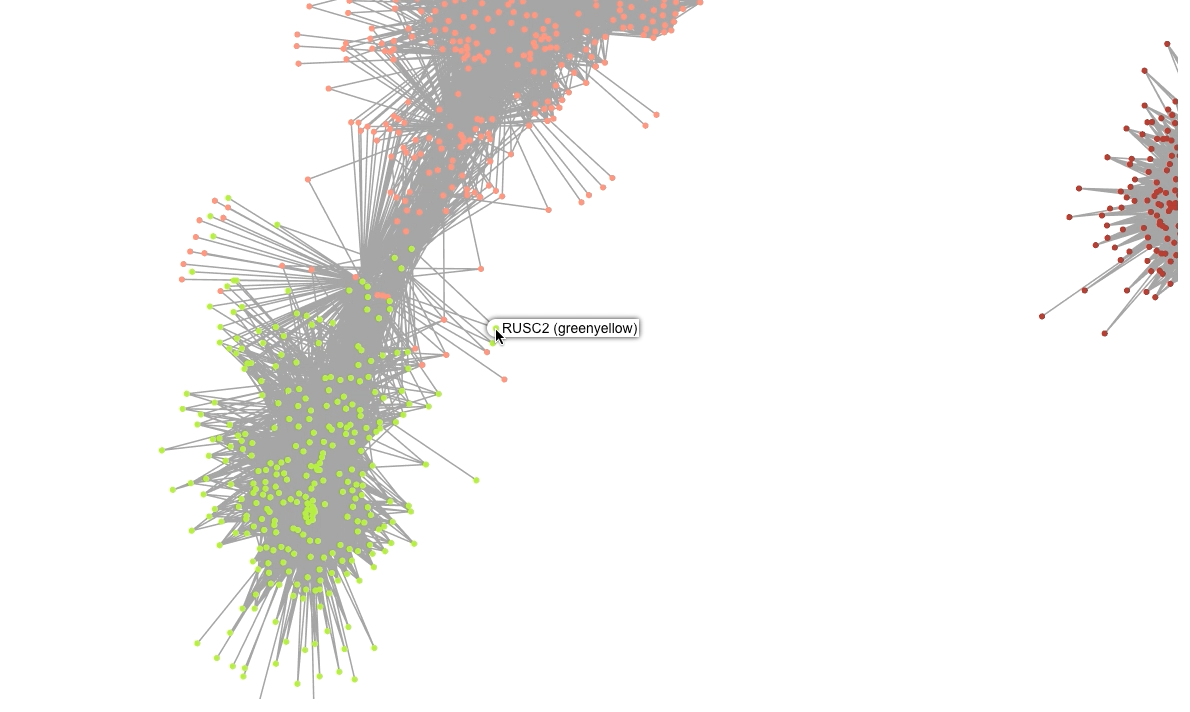
\includegraphics[width=2.7in]{figures/network.png}%
\label{fig_first_case}}
\hfil
\subfloat[A2: Module visualization.]{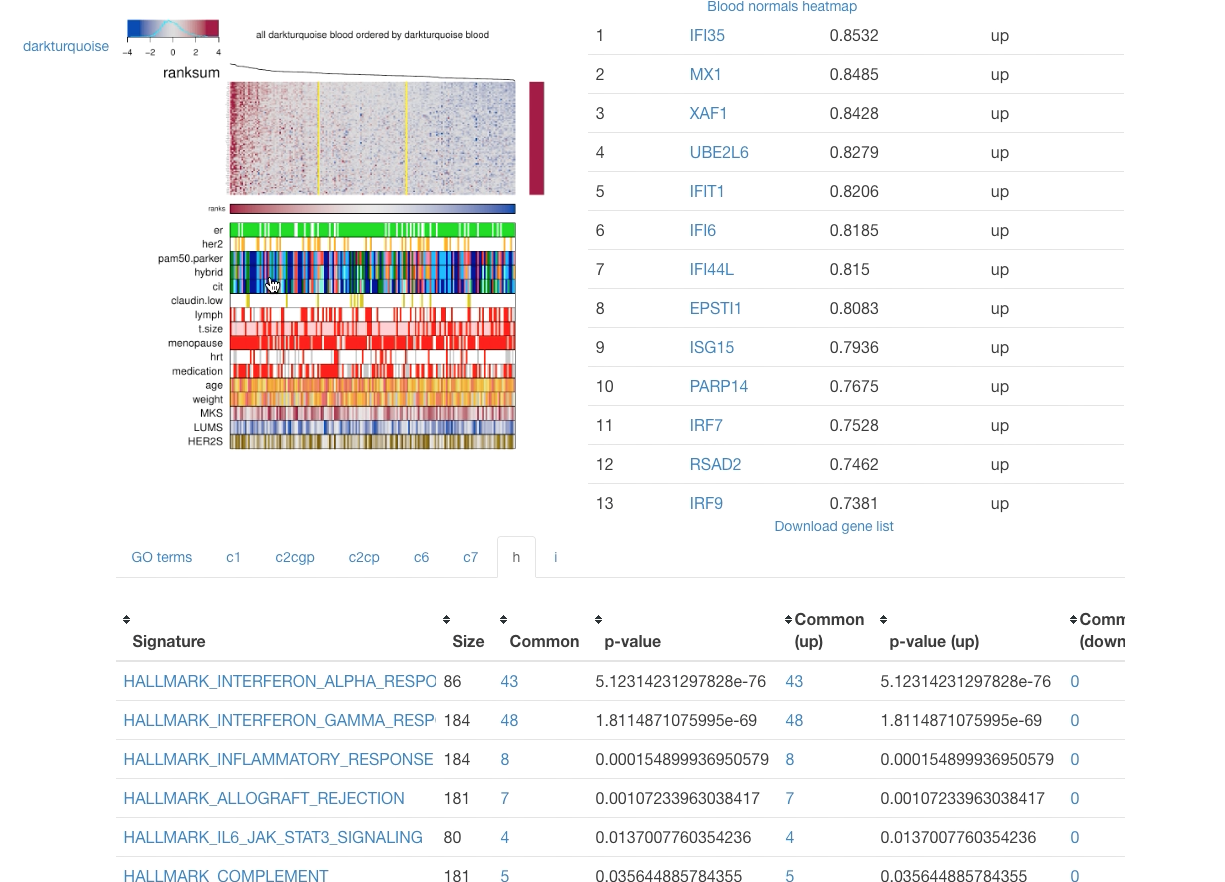
\includegraphics[width=2.5in]{figures/module.png}%
\label{fig_second_case}}
\hfil
\centering
\subfloat[A3: Visualization of ranksum.]{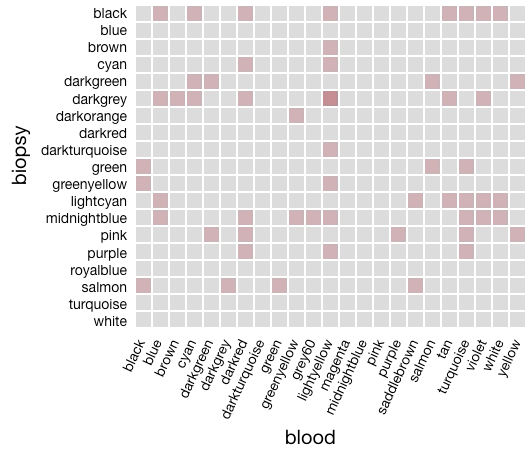
\includegraphics[width=2.5in]{figures/tissue-comp.png}%
\label{fig_first_case}}
\hfil
\subfloat[A4: Visualization of significant clinical variable
association]{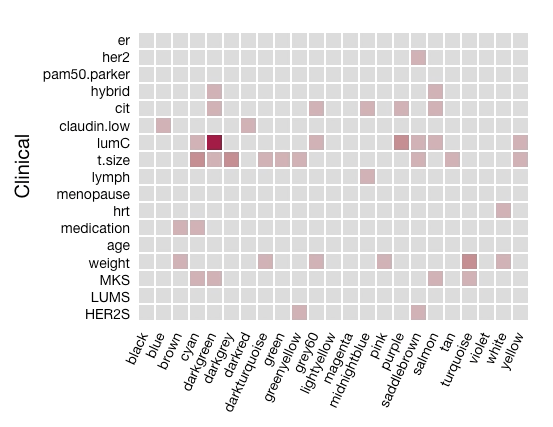
\includegraphics[width=2.8in]{figures/clinical-comp.png}%
\label{fig_second_case}}
\caption{Screenshots of the user interface in four of the six analysis tasks.
Note that we combine visualization frameworks for both JavaScript and R to
generate the visualizations. Specifically, sigmajs (a,
\protect\url{sigmajs.org}), ggplot2(b, \protect\url{ggplot2.org}), and D3 (c and
d, \protect\url{d3js.org})} 
\label{fig_sim}
\end{figure*}

\subsubsection*{Design and Implementation}
The MIxT application is designed as a modern application consisting of multiple
services that together provide an interactive web application. By composing an
application of a set of services we can substitute parts of the application
without re-writing the entire application. This type of architectural style is
called a microservices architecture and is popular in 'web-scale' systems. For
example if we want to use OpenCPU to interface with data analysis we can do so
by simply exchanging the Kvik R service with OpenCPU. Both services communicate
over HTTP and their interface is the same. 

From our initial analyses we built
an R package with functions to provide data and analysis to the different
analysis tasks. Using this design it is possible to either explore the data
through the web site or a local R session. 

To explore the co-expression relationship between genes we use an interactive
graph visualization build with Sigmajs\footnote{\url{sigmajs.org}}. We have
built visualization for both tissues, with graph sizes of 2705 nodes and 90 348
edges for the blood network, and 2066 nodes and 50 563 edges for the biopsy
network. The sigmajs visualization library has functionality for generating a
layout for large networks, but we generate this layout server-side to reduce the
computational load on the client. To generate this layout we use the GGally
package\footnote{\url{cran.r-project.org/web/packages/GGally}}. 

We have built modules for each tissue, and to explore gene sets associated with
genes in these modules, we provide module overview pages that show gene
expression visualized together with clinicopathological variables and gene set
analyses that describe the underlying functions of the module. 

We have used different metrics to link the modules from each tissue, ranksum and
gene overlap. To visualize the associations we use the
d3\footnote{\url{d3js.org}} library to build an interactive heatmap
visualization. 

To allow users to explore the relationship between clinical variables and the
computed modules, we built an interctive heatmap visualization that visualizes
the association between different metrics and each module. 



\section*{Conclusions}
